\chapter{Firewall and IDS/IPS} 

\begin{minipage}{0.6\textwidth}
\section{What is a Firewall?}
%	\vspace{-0.5cm}
A firewall acts as a protective barrier, much like a physical wall against fire. It is primarily a controlled connection point between networks with differing security levels. Its key functions include:
\begin{itemize}
    \item \textbf{Boundary Protection:} Serving as a network filter between trusted (internal) and untrusted (external) networks.
    \item \textbf{Compartmentalization:} Dividing network zones based on security levels to enforce stricter control.
\end{itemize}
\end{minipage} 
\hspace{0.5cm}
\begin{minipage}{0.4\textwidth}
    \centering
    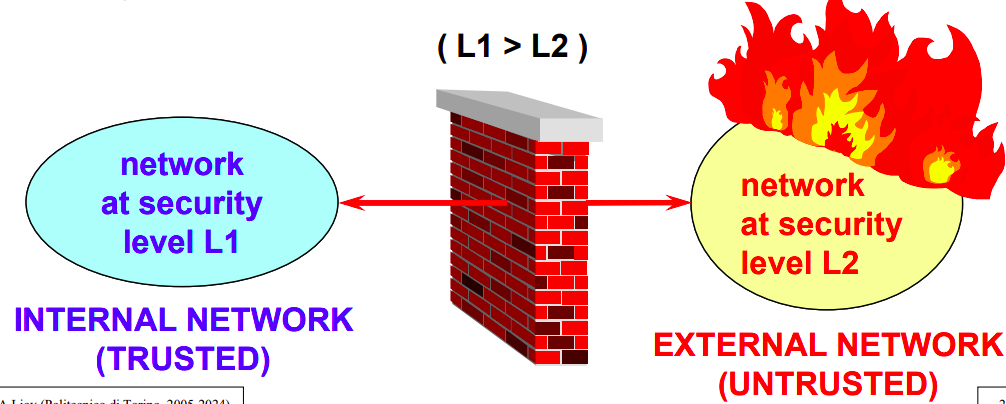
\includegraphics[width=\textwidth]{/home/lorenzo/Notes/Information System Security/images/Screenshot from 2024-11-21 15-09-40.png}
\end{minipage}

\section{Ingress vs Egress firewall}
Firewalls can be classified based on the direction of traffic they manage:
\begin{itemize}
    \item An \textbf{ingress firewall} focuses on incoming connections, typically regulating access to public services provided by the network or supporting exchanges initiated by internal users.
    \item An \textbf{egress firewall} monitors outgoing connections. It's typically used to check the activity of internal personnel [Works well for channel-based services (e.g., TCP applications) but faces challenges with stateless, message-based services (e.g., ICMP, UDP)].
\end{itemize}
\section{The three principles of the firewall}
\begin{enumerate}
    \item The firewall should be the only connection between the internal and external networks.
    \item Only the "authorized"  traffic is allowed to pass the firewall.
    \item The firewall itself must be secure against potential vulnerabilities.
\end{enumerate}
These principles were outlined by \textit{D.Cheswick, S.Bellovin}.

\section{Authorization policies}
\begin{itemize}
    \item \textbf{Permitlist/allowlist}: All that is not explicitly permitted, is forbidden. 
    \begin{itemize}
        \item It offers higher security but it's difficult to manage. 
    \end{itemize}
    \item \textbf{Blocklist/denylist}: All that is not explicitly forbidden, is permitted.
    \begin{itemize}
        \item It's less secure but it's more easy to manage. 
    \end{itemize}
\end{itemize}

\section{Basic components}
Firewalls include several key components that work together to provide security:
\begin{itemize}
    \item \textbf{Packet Filter/ Screening Router / Choke}: Filters traffic at the network level based on packet attributes such as IP headers and transport headers.
    \item \textbf{Bastion Host}: A secure system with auditing capabilities, often positioned to handle critical traffic.
    \item \textbf{Application Gateway (Proxy)}:  Acts on behalf of an application, managing access control and providing detailed packet inspection at the application level.
    \item \textbf{Dual-Homed Gateway}:  A system with two network interfaces and disabled routing, isolating internal and external networks. (In the way we can decide which packets are sent from a network to another).
\end{itemize}

\section{A which level the controls are made?}
Firewalls at higher levels provide more security but tend to be slower, while firewalls at lower levels offer less security but greater speed.
\begin{figure}[h]
    \centering
    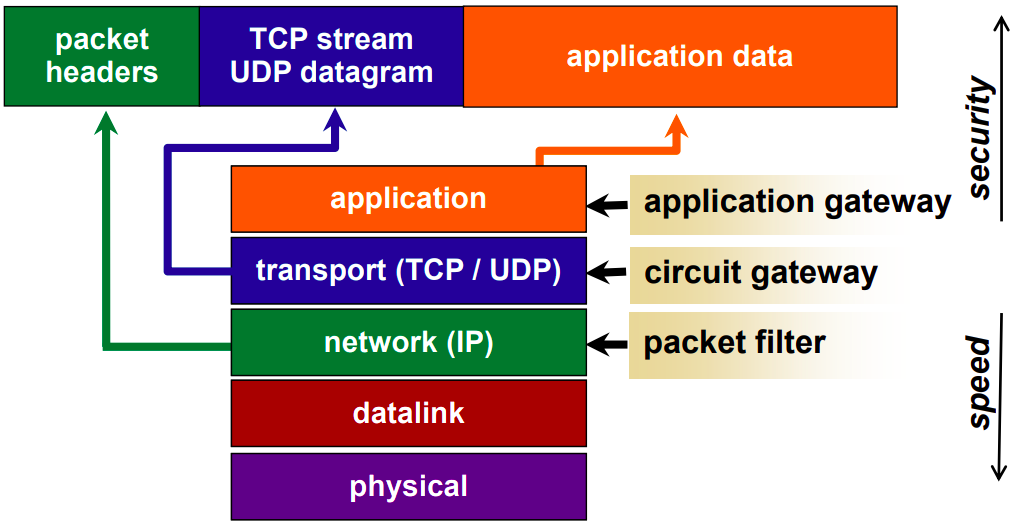
\includegraphics[width=0.5\textwidth]{/home/lorenzo/Notes/Information System Security/images/Screenshot from 2024-11-21 15-43-10.png}
\end{figure}
\begin{quotebox-yellow}{To undersand:}
    \textbf{security is better up} \(\rightarrow\) \textbf{speed is better down}\\
    \textbf{security is better down} \(\rightarrow\) \textbf{speed is better up}
\end{quotebox-yellow}

\section{Network-Level Controls}
Firewalls operate at various levels of the network stack applying different controls based on the type of firewall used:
\begin{itemize}
    \item \textbf{Packet Filters}: Operate at the network level, inspecting packet headers.
    \item \textbf{Stateful Packet Filters}: Track connection states for more dynamic filtering.ù
    \item \textbf{Circuit-Level Gateways / Proxies}: Work at the transport level, ensuring secure connection establishment.
    \item \textbf{Application-Level Gateways / Proxies}: Provide inspection and control at the application layer, often with more granular rules.
\end{itemize}

 \subsection{Packet filter}
 A packet filter inspects packets based on headers, such as IP and transport headers. These filters are traditionally available on routers and now in most OS. They allow for rules like permitting incoming connections to specific services (e.g., a web server) or limiting DNS queries from specific internal servers.

\definecolor{darkgreen}{rgb}{0.0, 0.39, 0.0}  % Custom dark green color
\begin{itemize}
    \item \textcolor{darkgreen}{\textbf{Pro:}} 
    \begin{itemize}
        \item Independent of applications, scalable, and cost-effective (available in many OS and routers).
        \item Good performance and low cost.
    \end{itemize}
    \item \textcolor{red}{\textbf{Cons:}} 
    \begin{itemize}
        \item Vulnerable to attacks like IP spoofing or fragmented packets.
        \item Difficult to support services using dynamically allocated ports (e.g. FTP).
        \item Complex configuration and hard to implement user authentication.
    \end{itemize}
\end{itemize}

\subsection{Circuit-Level Gateway}
A circuit-level gateway acts as a transport-level proxy, creating secure communication channels between client and server without inspecting the payload. It protects against Layer 3/Layer 4 attacks like IP fragmentation or TCP handshake exploits.
\begin{itemize}
    \item \textcolor{darkgreen}{\textbf{Pro:}} 
    \begin{itemize}
        \item Provides protection by isolating the server from attacks.
        \item Offers client authentication and eliminates many low-level attack vectors.
    \end{itemize}
    \item \textcolor{red}{\textbf{Cons:}} 
    \begin{itemize}
        \item Still shares many limitations of packet filters and requires modifications to the application for full functionality.
    \end{itemize}
\end{itemize}

\subsection{Application-Level Gateway}
An application-level gateway (or proxy) operates at the application layer, inspecting the payload of packets. These proxies often require modifications to client applications and can enhance security by checking the semantics of application data (e.g., HTTP methods) or performing peer authentication.
\begin{itemize}
    \item \textcolor{darkgreen}{\textbf{Pro:}} 
    \begin{itemize}
        \item Strong security against application vulnerabilities (e.g., buffer overflow attacks).
        \item Fine-grained access controls and the ability to mask internal IP addresses.
        \item May provide protection against attacks like buffer overflows.
        \item Not transparent to the client and may break the client-server model.
    \end{itemize}
    \item \textcolor{red}{\textbf{Cons:}} 
    \begin{itemize}
        \item Requires specific proxies for each application and can introduce delays when supporting new applications.
        \item High resource usage and lower performance due to user-mode operations.
    \end{itemize}
\end{itemize} 
Variants of application-level proxies include \textbf{transparent proxies}, which are less intrusive to clients, and \textbf{strong application proxies}, which focus on checking data semantics, not just syntax.

\subsection{HTTP Proxies}
An HTTP forward proxy is a server that acts as an intermediary or front-end for client requests. It receives requests from internal users and forwards them to the real external server (So it's a egress control).
\textbf{Benefits:}
\\\vspace{-0.8cm}
\begin{minipage}{0.65\textwidth}
	\vspace{0.5cm}
    \begin{itemize}
        \item \textbf{Shared Cache}: External web pages are cached, reducing load times for all internal users.
        \item \textbf{Authentication and Authorization}: Enforces user authentication and controls access for internal users.
        \item \textbf{Various controls} (e.g. allowed sites, transfer direction, data
        types, …).
    \end{itemize} 
\end{minipage} 
\hspace{0.4cm}
\begin{minipage}{0.3\textwidth}
    \centering
    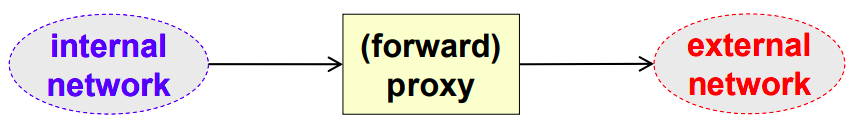
\includegraphics[width=1.2\textwidth]{/home/lorenzo/Notes/Information System Security/images/Screenshot from 2024-11-21 17-21-05.png}
\end{minipage}

\begin{quotebox-grey}{Type of Proxies}
    \begin{itemize}
        \item \textbf{Forward Proxy (HTTP Proxy)}: This type of proxy controls outgoing traffic from the internal network to the external one, enforcing access controls and caching content. It provides features like user authentication and authorization, content filtering, and bandwidth control.
        \item \textbf{Reverse Proxy (HTTP Reverse Proxy)}: A reverse proxy sits in front of web servers, providing additional services like load balancing, content inspection, TLS acceleration, and caching. It can obfuscate the internal server structure, improving security, and support performance optimizations like dynamic page feeding based on client speed.
    \end{itemize}
\end{quotebox-grey}

\begin{quotebox}[colframe=blue!10!white, colback=blue!5!white]{Reverse proxy: possibile configuration}
\begin{minipage}{0.5\textwidth}
    \underline{\textbf{Key components:}}
    \begin{itemize}
        \item \textbf{External Network (Red Cloud)}
        \item \textbf{Firewall}
        \item \textbf{DMZ (Demilitarized Zone)}: A buffer zone between external and internal networks where systems that interact with the external network are placed for added security.
        \item \textbf{Reverse Proxy}
        \item \textbf{Internal Network}: The secure area where your actual servers (e.g., serv1, serv2) reside.
    \end{itemize}    
\end{minipage} 
\hspace{0.5cm}
\begin{minipage}{0.45\textwidth}
    \centering
    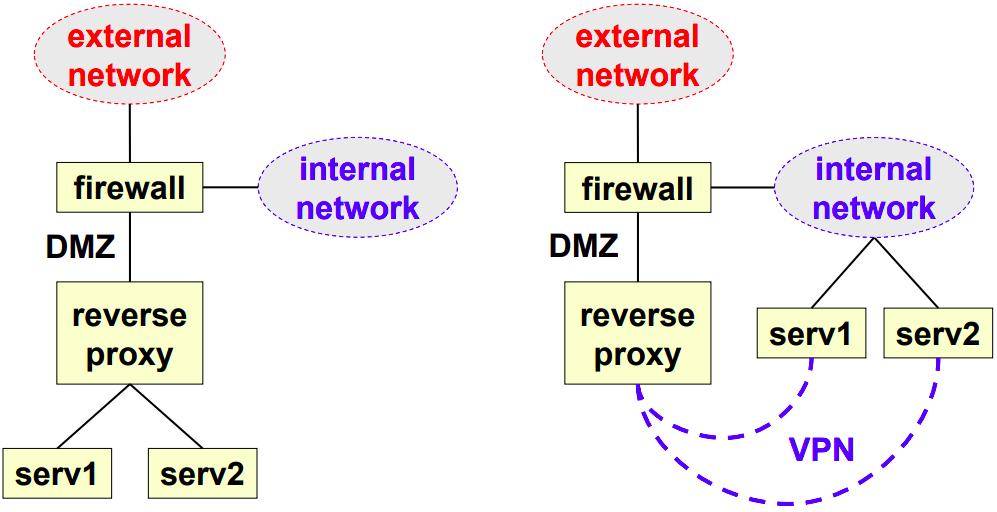
\includegraphics[width=\textwidth]{/home/lorenzo/Notes/Information System Security/images/Screenshot from 2024-11-21 17-38-55.png}
\end{minipage}
\\
\\\\
\underline{\textbf{How configurations work?}}
\\\\
\begin{minipage}[t]{0.45\textwidth}
   \textbf{Left configuration: Direct reverse proxy setup}
   \begin{itemize}
    \item \textbf{Flow:} External user \(\rightarrow\) Reverse Proxy \(\rightarrow\) Internal Servers (serv1, serv2).  
    \item \textbf{Benefits:} Internal servers are hidden and protected, while performance and security are improved.
   \end{itemize}
\end{minipage} 
\hspace{1cm}
\begin{minipage}[t]{0.45\textwidth}
   \textbf{Right Configuration: Reverse Proxy with VPN}
   \begin{itemize}
    \item \textbf{Flow}: External user \(\rightarrow\) Reverse Proxy \(\rightarrow\) Encrypted VPN connection \(\rightarrow\) Internal Servers (serv1, serv2).
    \item \textbf{Benefit}: Adds an extra layer of security through encryption for communication between the reverse proxy and internal servers.
   \end{itemize}
\end{minipage}
\end{quotebox}

\subsection{WAF (Web Application Firewall)}
A WAF is a module installed at a proxy (forward and/or reverse) to filter the application traffic. Filters the followings types of traffic:
\begin{itemize}
    \item HTTP commands.
    \item HTTP request/response headers.
    \item HTTP request/response content.
\end{itemize}
\begin{quotebox-grey}{Popular WAF example: \textbf{ModSecurity}}
    ModSecurity is a widely-used WAF plugin for web servers like Apache and NGINX, offering protection through predefined rules like the OWASP ModSecurity Core Rule Set (CRS).
\end{quotebox-grey}
\section{Firewall's Architectures}
\subsection{"Packet Filter" architecture}
\vspace{0.2cm}
\begin{quotebox-yellow}{What it does?}
This architecture uses a simple packet filter to screen traffic at both the IP and higher protocol levels (like TCP)
\end{quotebox-yellow}
\vspace{0.5cm}
\begin{minipage}{0.5\textwidth}
    \vspace{-0.5cm}
    \textbf{Key Points:}
    \begin{itemize}
        \item If implemented with a router then it's a "screening router" and there's \textbf{no need for extra dedicated hardware}.
        \item The packet filter element represents a \textbf{single point of failure}.
        \item \textbf{There's no need for proxies} or application modifications.
    \end{itemize}
\end{minipage}
\hfill
\begin{minipage}{0.5\textwidth}
    \centering
    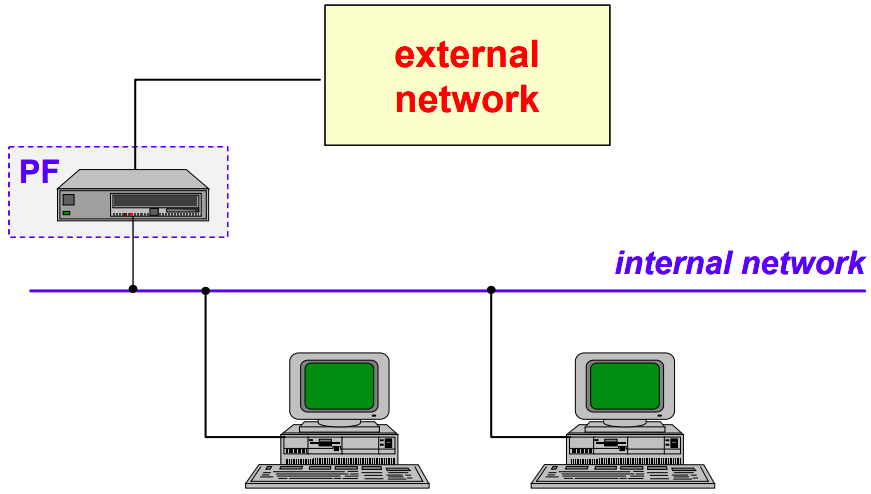
\includegraphics[width=0.8\textwidth]{/home/lorenzo/Notes/Information System Security/images/Screenshot from 2024-11-21 19-10-09.png}
\end{minipage}
\begin{center}
    \begin{quotebox-red}{Beware}
        Simple, cost-effective, but insecure!
        \end{quotebox-red}   
\end{center}
\vspace{0.5cm}
\subsection{"Dual-homed Gateway" architecture}
\vspace{0.2cm}
\begin{quotebox-yellow}{What it does?}
Uses a system with two network interfaces (hence "dual-homed") to provide a basic firewall between external and internal networks.
\end{quotebox-yellow}

\begin{minipage}{0.5\textwidth}
	\vspace{-2cm}
    \textbf{Key Points:}
    \begin{itemize}
        \item Easy to implement with small hardware requirements.
        \item The internal network can be masquerade.
    \end{itemize}
\end{minipage} 
\hfill
\begin{minipage}{0.5\textwidth}
    \centering
    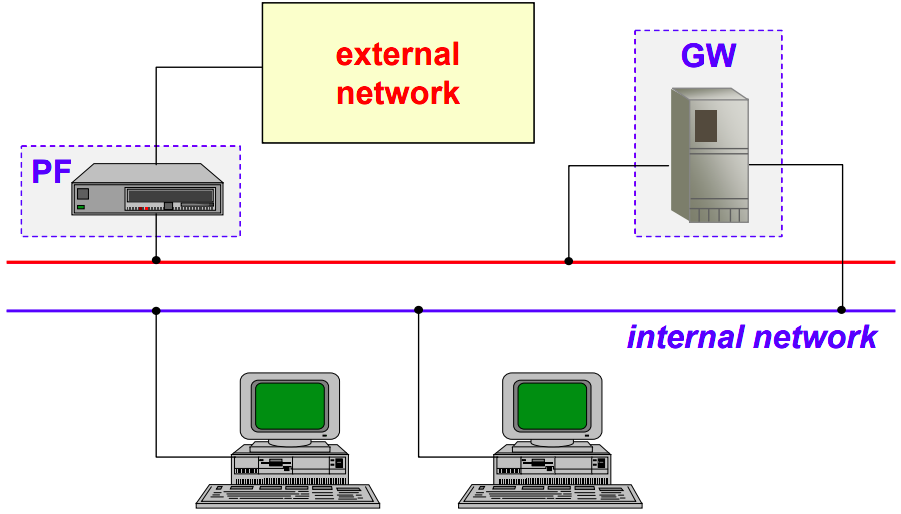
\includegraphics[width=0.8\textwidth]{/home/lorenzo/Notes/Information System Security/images/Screenshot from 2024-11-21 19-41-54.png}
\end{minipage}
\begin{center}
    \begin{quotebox-red}{Beware}
        Inflexible, with higher management overhead and reduced flexibility in handling complex network setups.
    \end{quotebox-red}   
\end{center}

\subsection{"Screened host" architecture}
\vspace{0.2cm}
\begin{quotebox-yellow}{What it does?}
    Uses two primary components: 
    \begin{itemize}
        \item \textbf{Router}
        \item \textbf{Bastion host}
    \end{itemize}
    This setup aims to provide enhanced security by controlling the flow of traffic between the internal and external networks.
\end{quotebox-yellow}

\begin{minipage}{0.5\textwidth}
	\vspace{-1.5cm}
    \textbf{Key Points:}
    \begin{itemize}
        \item Traffic from the internal network (INT) to external (EXT) is blocked unless it’s from the bastion host. Similarly, external traffic is blocked unless directed to the bastion.
        \item More flexible (skip control over some services / hosts)
    \end{itemize}
\end{minipage} 
\hfill
\begin{minipage}{0.5\textwidth}
    \centering
    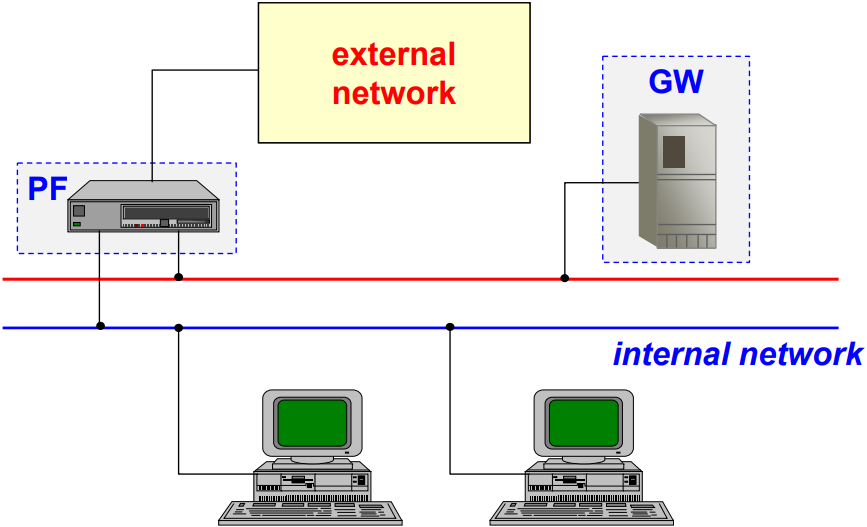
\includegraphics[width=0.8\textwidth]{
        /home/lorenzo/Notes/Information System Security/images/Screenshot from 2024-12-22 12-25-10.png}
\end{minipage}
\begin{center}
    \begin{quotebox-red}{Beware}
        \begin{itemize}
            \item \textbf{More Expensive and Complex} 
       to manage: Requires two systems (router + bastion host) instead of just one.
       \item \textbf{Limited Masking}: Only the host and protocols that go through the bastion host can be masked for security (such as hiding internal IP address or data). However, if the packet filter (PF) uses NAT, it can mask additional traffic and hide internal network details.
     \end{itemize}
    \end{quotebox-red}   
\end{center}

\subsection{"Screened subnet" architecture} 
\vspace{0.2cm}
\begin{quotebox-yellow}{What it does?}
A DMZ (De-Militarized Zone) is created between an internal network and a external network.
The DMZ  acts as a buffer zone to isolate external entities from the internal network, such as web servers or remote access points.
\end{quotebox-yellow}
\begin{minipage}{0.5\textwidth}
	%\vspace{-1.5cm}
    \textbf{Traffic flows:}
    \begin{itemize}
        \item The first firewall controls access from the external network to the DMZ, ensuring only authorized traffic can reach the public-facing systems.
        \item The second firewall restricts traffic from the DMZ to the internal network, allowing only specific and necessary connections.
    \end{itemize}
    \textcolor{darkgreen}{\textbf{It the most secure solution}} \textbf{because this setup hides the internal network from external users, reducing exposure to attacks.}
\end{minipage} 
\hfill
\begin{minipage}{0.5\textwidth}
    \centering
    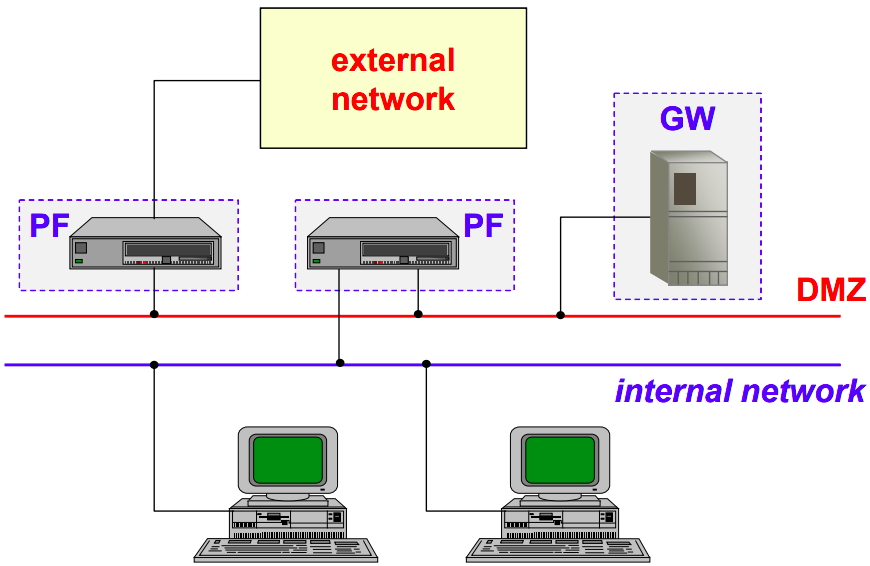
\includegraphics[width=0.8\textwidth]{
        /home/lorenzo/Notes/Information System Security/images/Screenshot from 2024-11-22 10-22-22.png}
\end{minipage}


\begin{center}
    \begin{quotebox-red}{Beware}
      \begin{itemize}
        \item \textbf{Higher cost} due to the additional hardware.
        \item \textbf{The DMZ is home not only to the gateway} but also to other host (typically the public servers).
      \end{itemize} 
    \end{quotebox-red}   
\end{center}
\newpage
\subsection{"Screened subnet" architecture (version 2)}
\vspace{0.2cm}
\begin{quotebox-yellow}{What it does?}
    In this version of the Screened Subnet architecture, the packet filters (\textbf{PF}) and gateway (\textbf{GW}) are merged into a single device that is called \textbf{AKA} ("three-legged firewall").
\end{quotebox-yellow}


\begin{minipage}{0.4\textwidth}
	%\vspace{-1.5cm}
    \textbf{Three-Legged design:}
    \begin{itemize}
        \item One interface connecting to the \textbf{External network} (untrusted).
        \item One interface connecting to the \textbf{Internal network} (trusted).
        \item One interface connecting to the DMZ (where public-facing services reside).
    \end{itemize}
\end{minipage} 
\hfill
\begin{minipage}{0.6\textwidth}
    \centering
    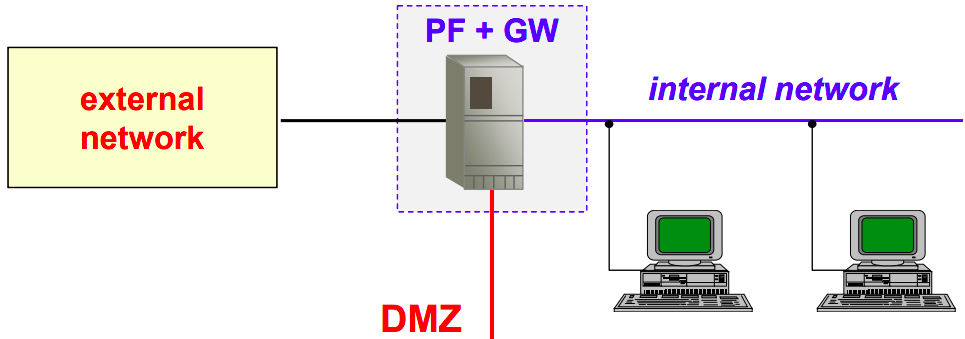
\includegraphics[width=0.8\textwidth]{
        /home/lorenzo/Notes/Information System Security/images/Screenshot from 2024-11-22 10-59-27.png}
\end{minipage}

\begin{center}
    \begin{quotebox-red}{Beware}
      It's \textcolor{darkgreen}{\textbf{more simple}} than the previous version but presents a \textbf{single point of failure}.
    \end{quotebox-red}   
\end{center}
\noindent{\color{gray!50}\rule{\textwidth}{0.5pt}}

\section{Local/Personal Firewall}
This image represents three different firewall configurations: \textbf{Network firewall}, \textbf{Local firewall} and \textbf{Personal firewall}. In the previous pages we have considered the network firewall, now let's start to analyze the Local/Personal firewall. \\
\begin{figure}[h]
    \centering
    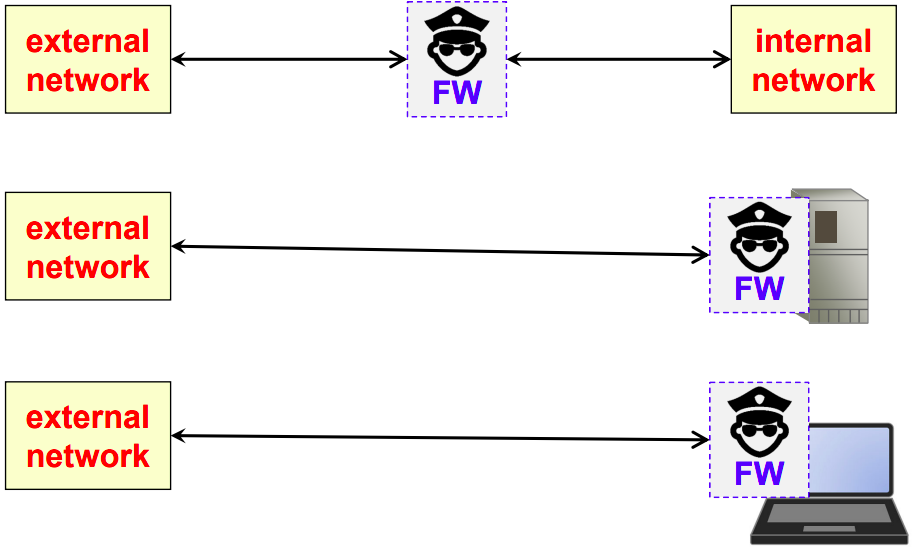
\includegraphics[width=0.5\textwidth]{/home/lorenzo/Notes/Information System Security/images/Screenshot from 2024-11-22 11-51-30.png}
\end{figure}
\\
\noindent
\textbf{A local or personal firewall} is installed directly on a device to protect it from unauthorized access or attacks. Unlike a normal network firewall, it may limit the PROCESSES that are permitted:
\begin{itemize}
    \item To open network channels towards other nodes (client behavior).
    \item To answer network requests (server behavior).
\end{itemize}

\noindent
These features make local firewalls essential for containing malware, blocking trojans, or preventing accidental misconfigurations. \textbf{However, in order to be effective, the firewall management MUST be separated from system management.}

\section{Protection offered by a firewall}
A firewall is 100\% effective only for attacks over/against blocked channels.
The other channels require other protection technique:
\begin{itemize}
    \item \textbf{VPNs}
    \item \textbf{intrusion detection systems (IDS)}
    \item \textbf{application-level protections}
\end{itemize}
\noindent{\color{gray!50}\rule{\textwidth}{0.5pt}}
\section{Intrusion Detection System (IDS)}
\begin{quotebox-yellow}{Definition}
An \textbf{Intrusion Detection System (IDS)}text is a security mechanism designed to:
\begin{itemize}
    \item identify actors using a system or a network without authorization (and their actions).
    \item  identify authorized actors who violate their privileges.
\end{itemize}
\textbf{Hypothesis}
\begin{itemize}
    \item The behavior “pattern” of non-authorized users differs from that of the authorized ones
\end{itemize}
\end{quotebox-yellow}

\subsection{IDS functional features}
\begin{itemize}
    \item \textbf{Passive IDS:} Observes and detects issues but doesn’t act to stop them.\\ \underline{Techniques:}
    \begin{itemize}
        \item Cryptographic checksums to detect changes in files.
        \item Pattern matching to identify attack signatures (e.g., malware signatures).
    \end{itemize}
    \item \textbf{Active IDS:} Monitors activity dynamically and reacts when thresholds are exceeded.\\ \underline{Techniques:}
    \begin{itemize}
        \item Tracks normal behavior to identify anomalies (\textbf{"learning"}).
        \item Gathers detailed statistics on traffic and actions (\textbf{text"monitoring"}).
        \item Triggers alerts or responses when unusual patterns occur (\textbf{"reaction}).
    \end{itemize}
\end{itemize}

\subsection{IDS topological features}
\begin{itemize}
    \item \textbf{HIDS (Host-Based IDS):} Monitors individual devices (hosts).
    \begin{itemize}
        \item Analyzes logs from the OS, services, or applications.
        \item Uses built-in OS tools to track internal activity.
    \end{itemize}
    \item \textbf{NIDS (Network-Based IDS):} Monitors traffic at the network level.
    \begin{itemize}
        \item Uses network traffic monitoring tools.
    \end{itemize}
\end{itemize}

\begin{quotebox-grey}{NIDS Architecture}
\underline{\textbf{Components:}}
\begin{itemize}
    \item \textbf{Sensor:} The frontline tool that analyzes traffic or logs looking for suspect patterns. Generates security alerts and can modify access controls (e.g., block traffic).
    \item \textbf{Director:} Coordinates sensors and manages a central database.
    \item \textbf{Message System:}  Ensures secure communication among IDS components.
\end{itemize}
\begin{minipage}{0.5\textwidth}
%	\vspace{-0.5cm}
\underline{\textbf{Workflow:}}
\begin{enumerate}
    \item Traffic from the external network enters through the firewall.
    \item (Net) sensors monitor traffic before it reaches the DMZ or internal network.
    \item Within the DMZ, host sensors monitor server activities.
    \item Traffic entering the internal network is further monitored by both host and network sensors.
    \item All sensors report suspicious activities to the IDS director.
    \item The IDS director consolidates this data and raises alerts or takes action if any patterns of intrusion or policy violations are detected.
\end{enumerate}
\end{minipage} 
\hspace{0.2cm}
\begin{minipage}{0.5\textwidth}
    \centering
    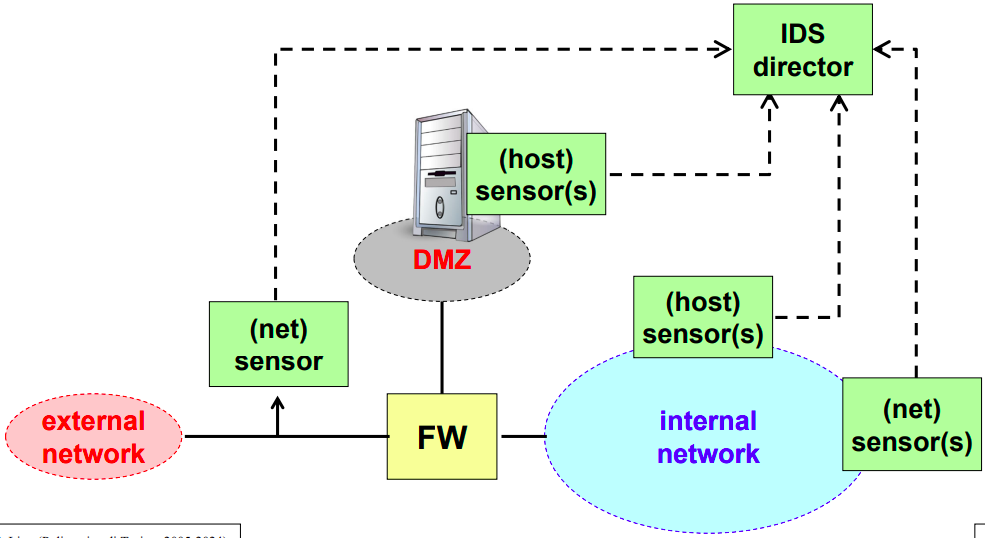
\includegraphics[width=\textwidth]{/home/lorenzo/Notes/Information System Security/images/Screenshot from 2024-11-22 14-41-40.png}
\end{minipage}
\end{quotebox-grey}

\section{Intrusion Prevention System (IPS)}
\vspace{0.2cm}
\begin{quotebox-yellow}{Definition}
An \textbf{Intrusion Prevention System (IPS)} is an advanced security technology (not a product) that identifies unauthorized activities like an IDS but actively blocks or mitigates them in real time (= IDS + distributed dynamic firewall).\\ Often, Intrusion Prevention Systems (IPS) are integrated with Intrusion Detection Systems (IDS) into a unified solution called \textbf{Intrusion Detection and Prevention System (IDPS)}
\end{quotebox-yellow}
\begin{center}
\begin{quotebox-red}{Why is it useful to merge IPS with IDS?}
    IPS already has some of IDS's features, such as detection capabilities. But merging IPS with IDS brings many advantages because:
    \begin{itemize}
        \item \textbf{IDS} excels in providing deep visibility into all network activity, including suspicious behavior that might not warrant immediate action.
        \item \textbf{IPS} actively blocks threats, but in doing so, it may not focus as much on monitoring benign-but-suspicious activities.
    \end{itemize}
\end{quotebox-red}
\end{center}
\noindent
\textcolor{red}{\textbf{N.B.}} IPS requires careful configuration and monitoring to balance its protective capabilities with the risk of blocking innocent traffic.

\section{Next-Generation Firewall (NGFW)}
A Next-Generation Firewall (NGFW) enhances traditional firewalls by offering features like \textbf{application identification}, regardless of the network port used, and traffic decryption. It can integrate with \textbf{authentication systems} such as Active Directory, enabling per-user and per-application security policies. Additionally, NGFWs provide advanced protection by \textbf{filtering traffic based on known vulnerabilities}, threats, and malware.

\section{Unified Threat Management (UTM)}
\textbf{Unified Threat Management (UTM) integrates multiple security features} such as firewalls, VPNs, anti-malware, content inspection, and IDPS into a single device. The goal is to simplify security management by consolidating various solutions, reducing complexity and costs, though the specific capabilities depend on the manufacturer.

\section{Honey pot / Honey net}
A honeypot is a decoy system designed to attract attackers and analyze their behavior, while a honeynet is a network of these decoy systems used to study both external and internal attacks. These tools help in identifying and understanding attack methods.
\begin{figure}[h]
    \centering
    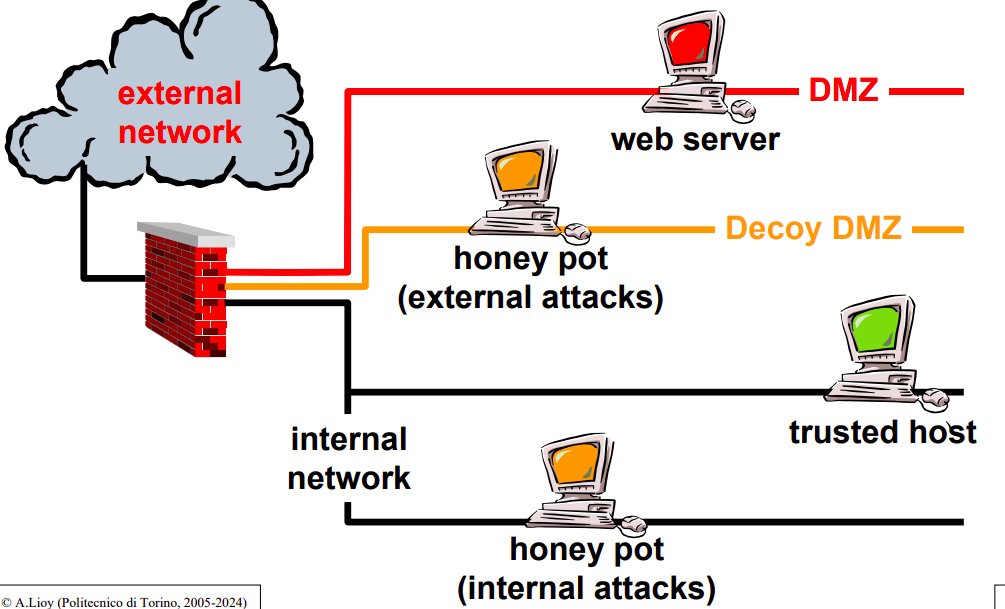
\includegraphics[width=0.4\textwidth]{/home/lorenzo/Notes/Information System Security/images/Screenshot from 2024-11-22 16-02-59.png}
\end{figure}




